% answers.tex —— 2009 年·普通高等学校招生考试·陕西卷·文科 · 参考答案与详细解析片段
% 由 tools/generate_projects.py 依来源总账自 2009/2009_数学真题_陕西文_试题.md + 2009/2009_数学真题_陕西文_解析正文.md + 2009/2009_数学真题_陕西文_答案要点.md 生成，勿手改（改源 MD 后重跑）


\begin{gktip}
固定候选 PDF 仅含题面，无答案、解析和评分标准，原页亦未标分值；以下为非官方编者独立推导，官方答案字段为空。分数、根号、上下标与三幅图均以 600 dpi 原页复核。
\end{gktip}

\begin{answer}
\gksolhead{1}{}

\textbf{题目}：

设不等式 $x^2-x\leqslant0$ 的解集为 $M$，函数 $f(x)=\ln(1-|x|)$ 的定义域为 $N$，则 $M\cap N$ 为（　）

（A）$[0,1)$

（B）$(0,1)$

（C）$[0,1]$

（D）$(-1,0]$

\Needspace{4\baselineskip}
\textbf{解析}

\Needspace{5\baselineskip}
$x^2-x\leqslant0$ 得 $0\leqslant x\leqslant1$，即 $M=[0,1]$。$1-|x|>0$ 得 $-1<x<1$，即 $N=(-1,1)$。故

\nopagebreak[4]
\[M\cap N=[0,1).\]

\gkanswer{答案：A。}

\end{answer}
\begin{answer}
\gksolhead{2}{}

\textbf{题目}：

若 $\tan\alpha=2$，则 $\dfrac{2\sin\alpha-\cos\alpha}{\sin\alpha+2\cos\alpha}$ 的值为（　）

（A）$0$

（B）$\dfrac34$

（C）$1$

（D）$\dfrac54$

\Needspace{4\baselineskip}
\textbf{解析}

\Needspace{5\baselineskip}
分子分母同除以 $\cos\alpha$：

\nopagebreak[4]
\[\frac{2\sin\alpha-\cos\alpha}{\sin\alpha+2\cos\alpha}
=\frac{2\tan\alpha-1}{\tan\alpha+2}
=\frac{4-1}{2+2}=\frac34.\]

\gkanswer{答案：B。}

\end{answer}
\begin{answer}
\gksolhead{3}{}

\textbf{题目}：

函数 $f(x)=\sqrt{2x-4}$（$x\geqslant4$）的反函数为（　）

（A）$f^{-1}(x)=\dfrac12x^2+4$（$x\geqslant0$）

（B）$f^{-1}(x)=\dfrac12x^2+4$（$x\geqslant2$）

（C）$f^{-1}(x)=\dfrac12x^2+2$（$x\geqslant0$）

（D）$f^{-1}(x)=\dfrac12x^2+2$（$x\geqslant2$）

\Needspace{4\baselineskip}
\textbf{解析}

\Needspace{5\baselineskip}
由 $y=\sqrt{2x-4}$ 得 $y\geqslant2$ 且 $y^2=2x-4$，故

\nopagebreak[4]
\[x=\frac{y^2+4}2=\frac12y^2+2.\]

交换 $x,y$ 得 $f^{-1}(x)=\dfrac12x^2+2$（$x\geqslant2$）。

\gkanswer{答案：D。}

\end{answer}
\begin{answer}
\gksolhead{4}{}

\textbf{题目}：

过原点且倾斜角为 $60^\circ$ 的直线被圆 $x^2+y^2-4y=0$ 所截得的弦长为（　）

（A）$\sqrt3$

（B）$2$

（C）$\sqrt6$

（D）$2\sqrt3$

\Needspace{4\baselineskip}
\textbf{解析}

\Needspace{5\baselineskip}
直线方程为 $y=\sqrt3x$，即 $\sqrt3x-y=0$。圆 $x^2+(y-2)^2=4$ 的圆心为 $(0,2)$，半径 $2$。圆心到直线距离

\nopagebreak[4]
\[d=\frac{|0-2|}{\sqrt{3+1}}=1.\]

\Needspace{5\baselineskip}
弦长

\nopagebreak[4]
\[2\sqrt{r^2-d^2}=2\sqrt{4-1}=2\sqrt3.\]

\gkanswer{答案：D。}

\end{answer}
\begin{answer}
\gksolhead{5}{}

\textbf{题目}：

某单位共有老、中、青职工 $430$ 人，其中青年职工 $160$ 人，中年职工人数是老年职工人数的 $2$ 倍．为了解职工身体状况，现采用分层抽样方法进行调查，在抽取的样本中有青年职工 $32$ 人，则该样本中的老年职工人数为（　）

（A）$9$

（B）$18$

（C）$27$

（D）$36$

\Needspace{4\baselineskip}
\textbf{解析}

\Needspace{5\baselineskip}
设老年职工 $x$ 人，则中年职工 $2x$ 人，青年 $160$ 人：

\nopagebreak[4]
\[x+2x+160=430,\qquad x=90.\]

\Needspace{5\baselineskip}
抽样比等于青年职工抽样比 $\dfrac{32}{160}=\dfrac15$，故老年职工样本数为

\nopagebreak[4]
\[90\times\frac15=18.\]

\gkanswer{答案：B。}

\end{answer}
\begin{answer}
\gksolhead{6}{}

\textbf{题目}：

若 $(1-2x)^{2009}=a_0+a_1x+\cdots+a_{2009}x^{2009}$（$x\in\mathbf R$），则 $\dfrac{a_1}2+\dfrac{a_2}{2^2}+\cdots+\dfrac{a_{2009}}{2^{2009}}$ 的值为（　）

（A）$2$

（B）$0$

（C）$-1$

（D）$-2$

\Needspace{4\baselineskip}
\textbf{解析}

\Needspace{5\baselineskip}
在恒等式 $(1-2x)^{2009}=a_0+a_1x+\cdots+a_{2009}x^{2009}$ 中令 $x=\dfrac12$：

\nopagebreak[4]
\[0=\left(1-2\cdot\frac12\right)^{2009}=a_0+\frac{a_1}2+\frac{a_2}{2^2}+\cdots+\frac{a_{2009}}{2^{2009}}.\]

又 $a_0=1$，故所求为 $-1$。

\gkanswer{答案：C。}

\end{answer}
\begin{answer}
\gksolhead{7}{}

\textbf{题目}：

“$m>n>0$”是“方程 $mx^2+ny^2=1$ 表示焦点在 $y$ 轴上的椭圆”的（　）

（A）充分而不必要条件

（B）必要而不充分条件

（C）充要条件

（D）既不充分也不必要条件

\Needspace{4\baselineskip}
\textbf{解析}

$mx^2+ny^2=1$ 即 $\dfrac{x^2}{1/m}+\dfrac{y^2}{1/n}=1$。因 $m>n>0$，有 $\dfrac1n>\dfrac1m>0$，长轴在 $y$ 轴上，故表示焦点在 $y$ 轴上的椭圆。

反之，若焦点在 $y$ 轴上，则 $\dfrac1n>\dfrac1m>0$，即 $m>n>0$。故为充要条件。

\gkanswer{答案：C。}

\end{answer}
\begin{answer}
\gksolhead{8}{}

\textbf{题目}：

在 $\triangle ABC$ 中，$M$ 是 $BC$ 的中点，$AM=1$，点 $P$ 在 $AM$ 上且满足 $\overrightarrow{AP}=2\overrightarrow{PM}$，则 $\overrightarrow{PA}\cdot(\overrightarrow{PB}+\overrightarrow{PC})$ 等于（　）

（A）$\dfrac49$

（B）$\dfrac43$

（C）$-\dfrac43$

（D）$-\dfrac49$

\Needspace{4\baselineskip}
\textbf{解析}

\Needspace{5\baselineskip}
以 $A$ 为原点，$\overrightarrow{AM}=\boldsymbol m$，$|\boldsymbol m|=1$。由 $\overrightarrow{AP}=2\overrightarrow{PM}$ 得 $P=\dfrac23\boldsymbol m$，故

\nopagebreak[4]
\[\overrightarrow{PA}=-\frac23\boldsymbol m.\]

\Needspace{5\baselineskip}
又 $M$ 为 $BC$ 中点，$\overrightarrow{PB}+\overrightarrow{PC}=2\overrightarrow{PM}$，而 $\overrightarrow{PM}=\dfrac13\boldsymbol m$，故

\nopagebreak[4]
\[\overrightarrow{PA}\cdot(\overrightarrow{PB}+\overrightarrow{PC})
=-\frac23\boldsymbol m\cdot\frac23\boldsymbol m
=-\frac49|\boldsymbol m|^2=-\frac49.\]

\gkanswer{答案：D。}

\end{answer}
\begin{answer}
\gksolhead{9}{}

\textbf{题目}：

从 $1,2,3,4,5,6,7$ 这七个数字中任取两个奇数和两个偶数，组成没有重复数字的四位数，其中奇数的个数为（　）

（A）$432$

（B）$288$

（C）$216$

（D）$108$

\Needspace{4\baselineskip}
\textbf{解析}

\Needspace{5\baselineskip}
奇数有 $1,3,5,7$ 四个，偶数有 $2,4,6$ 三个。选两个奇数、两个偶数的方法数为

\nopagebreak[4]
\[\mathrm C_4^2\mathrm C_3^2=6\times3=18.\]

\Needspace{5\baselineskip}
每组四个数字中恰有两个奇数，排在末位使数为奇数有 $2$ 种，其余三位任意排列有 $3!$ 种，故

\nopagebreak[4]
\[18\times2\times3!=18\times12=216.\]

\gkanswer{答案：C。}

\end{answer}
\begin{answer}
\gksolhead{10}{}

\textbf{题目}：

定义在 $\mathbf R$ 上的偶函数 $f(x)$ 满足：对任意的 $x_1,x_2\in[0,+\infty)$（$x_1\neq x_2$），有 $\dfrac{f(x_2)-f(x_1)}{x_2-x_1}<0$．则（　）

（A）$f(3)<f(-2)<f(1)$

（B）$f(1)<f(-2)<f(3)$

（C）$f(-2)<f(1)<f(3)$

（D）$f(3)<f(1)<f(-2)$

\Needspace{4\baselineskip}
\textbf{解析}

\Needspace{5\baselineskip}
条件说明 $f$ 在 $[0,+\infty)$ 上单调递减。又 $f$ 为偶函数，$f(-2)=f(2)$。由 $3>2>1\geqslant0$ 得

\nopagebreak[4]
\[f(3)<f(2)<f(1),\qquad f(3)<f(-2)<f(1).\]

\gkanswer{答案：A。}

\end{answer}
\begin{answer}
\gksolhead{11}{}

\textbf{题目}：

若正方体的棱长为 $\sqrt2$，则以该正方体各个面的中心为顶点的凸多面体的体积为（　）

（A）$\dfrac{\sqrt2}6$

（B）$\dfrac{\sqrt2}3$

（C）$\dfrac{\sqrt3}3$

（D）$\dfrac23$

\Needspace{4\baselineskip}
\textbf{解析}

\Needspace{5\baselineskip}
正方体各面中心构成正八面体，其六个顶点为 $\pm$ 各坐标轴方向上距中心 $\dfrac{\sqrt2}2$ 的点。正八面体可看作两个底面相同的正四棱锥，底面对角线长为 $\sqrt2$，故底面边长 $1$，每个棱锥高 $\dfrac{\sqrt2}2$。

\nopagebreak[4]
\[V=2\cdot\frac13\cdot1^2\cdot\frac{\sqrt2}2=\frac{\sqrt2}3.\]

\gkanswer{答案：B。}

\end{answer}
\begin{answer}
\gksolhead{12}{}

\textbf{题目}：

设曲线 $y=x^{n+1}$（$n\in\mathbf N^*$）在点 $(1,1)$ 处的切线与 $x$ 轴的交点的横坐标为 $x_n$，则 $x_1\cdot x_2\cdots x_n$ 的值为（　）

（A）$\dfrac1n$

（B）$\dfrac1{n+1}$

（C）$\dfrac n{n+1}$

（D）$1$

\Needspace{4\baselineskip}
\textbf{解析}

\Needspace{5\baselineskip}
$y'=(n+1)x^n$，在 $(1,1)$ 处切线斜率 $n+1$，切线为

\nopagebreak[4]
\[y-1=(n+1)(x-1).\]

\Needspace{5\baselineskip}
令 $y=0$：

\nopagebreak[4]
\[-1=(n+1)(x-1),\qquad x=1-\frac1{n+1}=\frac n{n+1}.\]

\Needspace{5\baselineskip}
故

\nopagebreak[4]
\[x_1x_2\cdots x_n=\frac12\cdot\frac23\cdots\frac n{n+1}=\frac1{n+1}.\]

\gkanswer{答案：B。}

\end{answer}
\begin{answer}
\gksolhead{13}{}

\textbf{题目}：

设等差数列 $\{a_n\}$ 的前 $n$ 项和为 $S_n$，若 $a_6=S_3=12$，则 $\{a_n\}$ 的通项 $a_n=$ $\underline{\qquad}$．

\Needspace{4\baselineskip}
\textbf{解析}

\Needspace{5\baselineskip}
设首项 $a_1$、公差 $d$。由 $a_6=12$：

\nopagebreak[4]
\[a_1+5d=12.\]

\Needspace{5\baselineskip}
由 $S_3=12$：

\nopagebreak[4]
\[3a_1+\frac{3\cdot2}2d=12,\qquad a_1+d=4.\]

\Needspace{5\baselineskip}
两式相减得 $4d=8$，$d=2$，$a_1=2$。故

\nopagebreak[4]
\[a_n=2+(n-1)\cdot2=2n.\]

\gkanswer{答案：$2n$。}

\end{answer}
\begin{answer}
\gksolhead{14}{}

\textbf{题目}：

设 $x$，$y$ 满足约束条件 $\begin{cases}x+y\geqslant1,\\ x-y\geqslant-1,\\ 2x-y\leqslant2,\end{cases}$ 目标函数 $z=x+2y$ 的最小值是$\underline{\qquad}$，最大值是$\underline{\qquad}$．

\Needspace{4\baselineskip}
\textbf{解析}

\Needspace{5\baselineskip}
三条边界两两相交于

\nopagebreak[4]
\[(0,1),\quad (1,0),\quad (3,4).\]

\Needspace{5\baselineskip}
逐点计算 $z=x+2y$：

\nopagebreak[4]
\[z(0,1)=2,\qquad z(1,0)=1,\qquad z(3,4)=11.\]

可行域为以此三点为顶点的三角形，故最小值为 $1$，最大值为 $11$。

\gkanswer{答案：$1$；$11$。}

\end{answer}
\begin{answer}
\gksolhead{15}{}

\textbf{题目}：

如图，球 $O$ 的半径为 $2$，圆 $O_1$ 是一小圆，$O_1O=\sqrt2$，$A$，$B$ 是圆 $O_1$ 上两点．若 $A$，$B$ 两点间的球面距离为 $\dfrac{2\pi}3$，则 $\angle AO_1B=$ $\underline{\qquad}$．
\nopagebreak[4]
\begin{center}% 2009 年陕西卷文科第 15 题：球 O 与小圆 O1。
% 来源 PDF：普通高考/2009/2009陕西文.pdf，SHA-256 c4760285004d01aee97af7821783660b08339cca3a3fc8645052f11001ba586a。
% 原页：第 1 页（A3 三栏）第 2 栏中部，书页码 551。
% 重绘依据：球半径 2、OO1=√2，按 1 单位=1.4cm 绘制；小圆用椭圆表示，A、B 在小圆前缘。
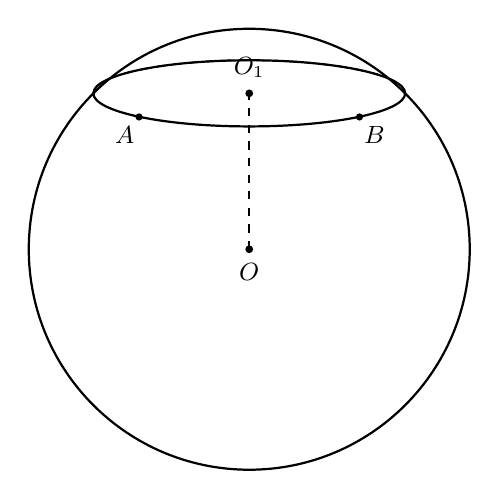
\begin{tikzpicture}[semithick, every node/.style={inner sep=1.4pt, font=\small}]
  % 球
  \draw[thick] (0,0) circle (2.8);
  % 小圆（投影为椭圆）
  \draw[thick] (0,1.98) ellipse (1.98 and 0.42);
  \draw[dashed] (1.98,1.98) arc (0:180:1.98 and 0.42);
  % 球心与小圆圆心
  \fill (0,0) circle (1.4pt);
  \fill (0,1.98) circle (1.4pt);
  \draw[dashed] (0,0) -- (0,1.98);
  % A、B
  \fill (-1.40,1.68) circle (1.3pt);
  \fill (1.40,1.68) circle (1.3pt);
  % 标注
  \node[below] at (0,-0.12) {$O$};
  \node[above] at (0,2.12) {$O_1$};
  \node[below left] at (-1.40,1.62) {$A$};
  \node[below right] at (1.40,1.62) {$B$};
\end{tikzpicture}
\end{center}
\nopagebreak[4]
\Needspace{4\baselineskip}
\textbf{解析}

\Needspace{5\baselineskip}
球半径 $R=2$，球面距离 $\dfrac{2\pi}3=R\theta$，故球心角 $\theta=\dfrac\pi3$。弦

\nopagebreak[4]
\[AB=2R\sin\frac\theta2=4\sin\frac\pi6=2.\]

\Needspace{5\baselineskip}
小圆半径

\nopagebreak[4]
\[O_1A=\sqrt{R^2-OO_1^2}=\sqrt{4-2}=\sqrt2.\]

\Needspace{5\baselineskip}
在 $\triangle AO_1B$ 中，

\nopagebreak[4]
\[AB=2O_1A\sin\frac{\angle AO_1B}2
\Longrightarrow 2=2\sqrt2\sin\frac{\angle AO_1B}2,\]

故 $\sin\dfrac{\angle AO_1B}2=\dfrac{\sqrt2}2$，$\angle AO_1B=\dfrac\pi2$。

\gkanswer{答案：$\dfrac\pi2$。}

\end{answer}
\begin{answer}
\gksolhead{16}{}

\textbf{题目}：

某班有 $36$ 名同学参加数学、物理、化学课外探究小组，每名同学至多参加两个小组，已知参加数学、物理、化学小组的人数分别为 $26$，$15$，$13$，同时参加数学和物理小组的有 $6$ 人，同时参加物理和化学小组的有 $4$ 人，则同时参加数学和化学小组的有$\underline{\qquad}$人．

\Needspace{4\baselineskip}
\textbf{解析}

\Needspace{5\baselineskip}
设同时参加数学和化学小组的有 $x$ 人。因每人至多参加两个小组，三个小组人数之和中，同时参加两个小组的人各被计两次，故总人数

\nopagebreak[4]
\[36=26+15+13-6-4-x.\]

即 $36=44-x$，$x=8$。

\gkanswer{答案：$8$。}

\end{answer}
\begin{answer}
\gksolhead{17}{}

\textbf{题目}：

已知函数 $f(x)=A\sin(\omega x+\varphi)$，$x\in\mathbf R$（其中 $A>0$，$\omega>0$，$0<\varphi<\dfrac\pi2$）的周期为 $\pi$，且图象上一个最低点为 $M\left(\dfrac{2\pi}3,-2\right)$．

（1）求 $f(x)$ 的解析式；

（2）当 $x\in\left[0,\dfrac\pi{12}\right]$ 时，求 $f(x)$ 的最值．

\Needspace{4\baselineskip}
\textbf{解析}

\Needspace{5\baselineskip}
（1）周期 $\dfrac{2\pi}\omega=\pi$，故 $\omega=2$。最低点纵坐标为 $-2$，故 $A=2$。由 $M\left(\dfrac{2\pi}3,-2\right)$ 在图象上：

\nopagebreak[4]
\[\sin\left(2\cdot\frac{2\pi}3+\varphi\right)=-1,\]

\nopagebreak[4]
\[\frac{4\pi}3+\varphi=\frac{3\pi}2+2k\pi,\qquad \varphi=\frac\pi6+2k\pi.\]

\Needspace{5\baselineskip}
由 $0<\varphi<\dfrac\pi2$，取 $\varphi=\dfrac\pi6$。故

\nopagebreak[4]
\[f(x)=2\sin\left(2x+\frac\pi6\right).\]

\Needspace{5\baselineskip}
（2）当 $x\in\left[0,\dfrac\pi{12}\right]$ 时，

\nopagebreak[4]
\[2x+\frac\pi6\in\left[\frac\pi6,\frac\pi3\right],\]

\Needspace{5\baselineskip}
故 $\sin\left(2x+\dfrac\pi6\right)\in\left[\dfrac12,\dfrac{\sqrt3}2\right]$，

\nopagebreak[4]
\[f(x)\in[1,\sqrt3].\]

最小值 $1$ 在 $x=0$ 取得，最大值 $\sqrt3$ 在 $x=\dfrac\pi{12}$ 取得。

\gkanswer{答案：（1）$f(x)=2\sin\left(2x+\dfrac\pi6\right)$；（2）最小值 $1$，最大值 $\sqrt3$。}

\end{answer}
\begin{answer}
\gksolhead{18}{}

\textbf{题目}：

据统计，某食品企业一个月内被消费者投诉的次数为 $0$，$1$，$2$ 的概率分别为 $0.4$，$0.5$，$0.1$．

（1）求该企业在一个月内共被消费者投诉不超过 $1$ 次的概率；

（2）假设一月份与二月份被消费者投诉的次数互不影响，求该企业在这两个月内共被消费者投诉 $2$ 次的概率．

\Needspace{4\baselineskip}
\textbf{解析}

\Needspace{5\baselineskip}
（1）

\nopagebreak[4]
\[P(\xi\leqslant1)=P(\xi=0)+P(\xi=1)=0.4+0.5=0.9.\]

\Needspace{5\baselineskip}
（2）两个月投诉总数为 $2$ 的情形为 $(0,2)$、$(1,1)$、$(2,0)$，故

\nopagebreak[4]
\[P=0.4\times0.1+0.5\times0.5+0.1\times0.4
=0.04+0.25+0.04=0.33.\]

\gkanswer{答案：（1）$0.9$；（2）$0.33$。}

\end{answer}
\begin{answer}
\gksolhead{19}{}

\textbf{题目}：

如图，在直三棱柱 $ABC-A_1B_1C_1$ 中，$AB=1$，$AC=AA_1=\sqrt3$，$\angle ABC=60^\circ$．

（1）证明：$AB\perp A_1C$；

（2）求二面角 $A-A_1C-B$ 的大小．
\nopagebreak[4]
\begin{center}% 2009 年陕西卷文科第 19 题：直三棱柱 ABC-A1B1C1（AB=1，AC=AA1=√3，∠ABC=60°）。
% 来源 PDF：普通高考/2009/2009陕西文.pdf，SHA-256 c4760285004d01aee97af7821783660b08339cca3a3fc8645052f11001ba586a。
% 原页：第 1 页（A3 三栏）第 3 栏下部，书页码 551。
% 重绘依据：B(0,0,0)、A(1,0,0)、C(1,√3,0)、A1(1,0,√3)，投影 (x,y,z)->(x+0.35y, 1.6z+0.25y)。
%   A1C 为解题辅助线，画虚线；其余棱按直三棱柱绘制。
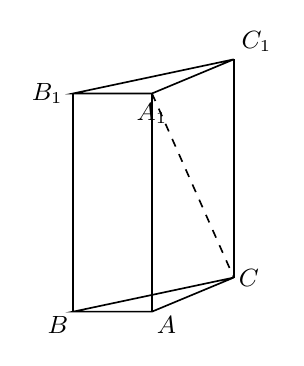
\begin{tikzpicture}[semithick, every node/.style={inner sep=1.5pt, font=\small}]
  \coordinate (B)  at (0.000,0.000);
  \coordinate (A)  at (1.000,0.000);
  \coordinate (C)  at (2.039,0.433);
  \coordinate (B1) at (0.000,2.771);
  \coordinate (A1) at (1.000,2.771);
  \coordinate (C1) at (2.039,3.204);

  % 棱
  \draw (B) -- (A) -- (C) -- cycle;
  \draw (B1) -- (A1) -- (C1) -- cycle;
  \draw (A) -- (A1);
  \draw (B) -- (B1);
  \draw (C) -- (C1);
  % 辅助线
  \draw[dashed] (A1) -- (C);

  % 标注
  \node[below left] at (B) {$B$};
  \node[below right] at (A) {$A$};
  \node[right] at (C) {$C$};
  \node[left=2pt] at (B1) {$B_1$};
  \node[below=2pt] at (A1) {$A_1$};
  \node[above right=1pt] at (C1) {$C_1$};
\end{tikzpicture}
\end{center}
\nopagebreak[4]
\Needspace{4\baselineskip}
\textbf{解析}

\Needspace{5\baselineskip}
（1）由 $AB=1$，$AC=\sqrt3$，$\angle ABC=60^\circ$，设 $BC=a$，由余弦定理

\nopagebreak[4]
\[AC^2=AB^2+BC^2-2AB\cdot BC\cos60^\circ,\]

\nopagebreak[4]
\[3=1+a^2-a,\qquad a^2-a-2=0,\qquad a=2.\]

\Needspace{5\baselineskip}
以 $B$ 为原点，$BA$ 为 $x$ 轴，平面 $ABC$ 为 $xOy$ 平面建系：

\nopagebreak[4]
\[B(0,0,0),\quad A(1,0,0),\quad C(1,\sqrt3,0),\quad A_1(1,0,\sqrt3).\]

\Needspace{5\baselineskip}
于是

\nopagebreak[4]
\[\overrightarrow{AB}=(-1,0,0),\qquad \overrightarrow{A_1C}=(0,\sqrt3,-\sqrt3),\]

\nopagebreak[4]
\[\overrightarrow{AB}\cdot\overrightarrow{A_1C}=0,\]

故 $AB\perp A_1C$。

（2）平面 $AA_1C$ 过 $A(1,0,0)$，$A_1(1,0,\sqrt3)$，$C(1,\sqrt3,0)$，其方程为 $x=1$，法向量 $\boldsymbol n_1=(1,0,0)$。

\Needspace{5\baselineskip}
平面 $BA_1C$ 的法向量

\nopagebreak[4]
\[\boldsymbol n_2=\overrightarrow{BA_1}\times\overrightarrow{BC}
=(1,0,\sqrt3)\times(1,\sqrt3,0)
=(-3,\sqrt3,\sqrt3).\]

\Needspace{5\baselineskip}
设二面角为 $\theta$，则

\nopagebreak[4]
\[\cos\theta=\frac{|\boldsymbol n_1\cdot\boldsymbol n_2|}{|\boldsymbol n_1||\boldsymbol n_2|}
=\frac3{\sqrt{15}}=\frac{\sqrt{15}}5.\]

故 $\theta=\arccos\dfrac{\sqrt{15}}5$，$\tan\theta=\dfrac{\sqrt6}3$。

\gkanswer{答案：（1）证明见解析；（2）$\arccos\dfrac{\sqrt{15}}5$（正切 $\dfrac{\sqrt6}3$）。}

\end{answer}
\begin{answer}
\gksolhead{20}{}

\textbf{题目}：

已知函数 $f(x)=x^3-3ax-1$，$a\neq0$．

（1）求 $f(x)$ 的单调区间；

（2）若 $f(x)$ 在 $x=-1$ 处取得极值，直线 $y=m$ 与 $y=f(x)$ 的图象有三个不同的交点，求 $m$ 的取值范围．

\Needspace{4\baselineskip}
\textbf{解析}

\Needspace{5\baselineskip}
（1）

\nopagebreak[4]
\[f'(x)=3x^2-3a=3(x^2-a).\]

若 $a<0$，则 $f'(x)>0$ 对一切 $x$ 成立，$f$ 在 $\mathbf R$ 上递增。

若 $a>0$，令 $f'(x)=0$ 得 $x=\pm\sqrt a$。当 $x<-\sqrt a$ 或 $x>\sqrt a$ 时 $f'(x)>0$；当 $-\sqrt a<x<\sqrt a$ 时 $f'(x)<0$。故增区间为 $(-\infty,-\sqrt a)$ 与 $(\sqrt a,+\infty)$，减区间为 $(-\sqrt a,\sqrt a)$。

\Needspace{5\baselineskip}
（2）$x=-1$ 为极值点，故

\nopagebreak[4]
\[f'(-1)=3-3a=0,\qquad a=1.\]

\Needspace{5\baselineskip}
此时 $f(x)=x^3-3x-1$，$f'(x)=3(x^2-1)$。极大值

\nopagebreak[4]
\[f(-1)=-1+3-1=1,\]

\Needspace{5\baselineskip}
极小值

\nopagebreak[4]
\[f(1)=1-3-1=-3.\]

\Needspace{5\baselineskip}
三次函数图象与水平线 $y=m$ 有三个不同交点，当且仅当 $m$ 严格介于极小值与极大值之间：

\nopagebreak[4]
\[-3<m<1.\]

\gkanswer{答案：（1）$a<0$ 时在 $\mathbf R$ 上递增；$a>0$ 时增区间 $(-\infty,-\sqrt a)$、$(\sqrt a,+\infty)$，减区间 $(-\sqrt a,\sqrt a)$；（2）$-3<m<1$。}

\end{answer}
\begin{answer}
\gksolhead{21}{}

\textbf{题目}：

已知数列 $\{a_n\}$ 满足 $a_1=1$，$a_2=2$，$a_{n+2}=\dfrac{a_n+a_{n+1}}2$，$n\in\mathbf N^*$．

（1）令 $b_n=a_{n+1}-a_n$，证明：$\{b_n\}$ 是等比数列；

（2）求 $\{a_n\}$ 的通项公式．

\Needspace{4\baselineskip}
\textbf{解析}

\Needspace{5\baselineskip}
（1）由 $a_{n+2}=\dfrac{a_n+a_{n+1}}2$，

\nopagebreak[4]
\[b_{n+1}=a_{n+2}-a_{n+1}
=\frac{a_n+a_{n+1}}2-a_{n+1}
=\frac{a_n-a_{n+1}}2=-\frac12b_n.\]

又 $b_1=a_2-a_1=1\neq0$，故 $\{b_n\}$ 是首项 $1$、公比 $-\dfrac12$ 的等比数列。

\Needspace{5\baselineskip}
（2）由（1），

\nopagebreak[4]
\[b_n=\left(-\frac12\right)^{n-1}.\]

\Needspace{5\baselineskip}
于是

\nopagebreak[4]
\[a_n=a_1+\sum_{k=1}^{n-1}b_k
=1+\frac{1-\left(-\frac12\right)^{n-1}}{1+\frac12}
=1+\frac23\left[1-\left(-\frac12\right)^{n-1}\right],\]

\Needspace{5\baselineskip}
即

\nopagebreak[4]
\[a_n=\frac53-\frac23\left(-\frac12\right)^{n-1}.\]

检验 $n=1,2$：$a_1=\dfrac53-\dfrac23=1$，$a_2=\dfrac53+\dfrac13=2$，与题设一致。

\gkanswer{答案：（1）证明见解析；（2）$a_n=\dfrac53-\dfrac23\left(-\dfrac12\right)^{n-1}$。}

\end{answer}
\begin{answer}
\gksolhead{22}{}

\textbf{题目}：

已知双曲线 $C$ 的方程为 $\dfrac{y^2}{a^2}-\dfrac{x^2}{b^2}=1$（$a>0$，$b>0$），离心率 $e=\dfrac{\sqrt5}2$，顶点到渐近线的距离为 $\dfrac{2\sqrt5}5$．

（1）求双曲线 $C$ 的方程；

（2）如图，$P$ 是双曲线 $C$ 上一点，$A$，$B$ 两点在双曲线 $C$ 的两条渐近线上，且分别位于第一、二象限，若 $\overrightarrow{AP}=\lambda\overrightarrow{PB}$，$\lambda\in\left[\dfrac13,2\right]$，求 $\triangle AOB$ 面积的取值范围．
\nopagebreak[4]
\begin{center}% 2009 年陕西卷文科第 22 题：双曲线 y^2/4 - x^2 = 1、两条渐近线与点 A、B、P。
% 来源 PDF：普通高考/2009/2009陕西文.pdf，SHA-256 c4760285004d01aee97af7821783660b08339cca3a3fc8645052f11001ba586a。
% 原页：第 2 页（A3 三栏）第 3 栏上部，书页码 552。
% 重绘依据：按 y^2/4-x^2=1 与渐近线 y=±2x 等比绘制；取 λ=1/2 的构型
%   A(1.5,3)、B(-0.75,1.5)、P(0.75,2.5)，P 在双曲线上。
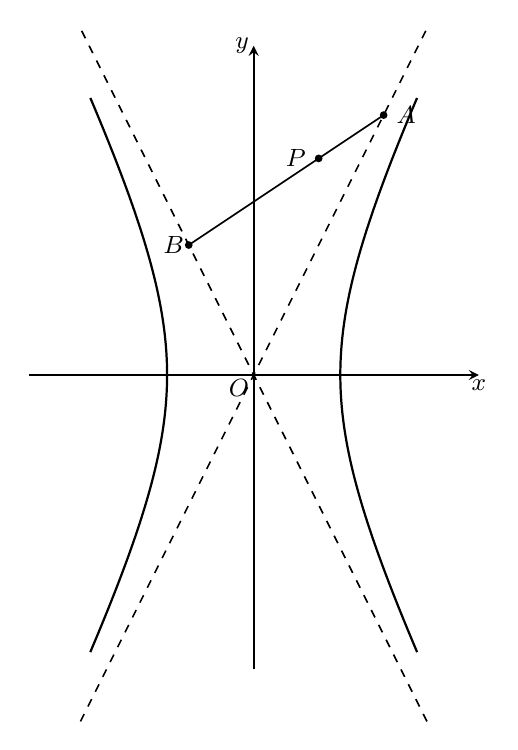
\begin{tikzpicture}[semithick, x=1.1cm, y=1.1cm, every node/.style={inner sep=1.4pt, font=\small}]
  % 坐标轴
  \draw[-stealth] (-2.6,0) -- (2.6,0) node[below] {$x$};
  \draw[-stealth] (0,-3.4) -- (0,3.8) node[left] {$y$};
  \node[below left] at (0,0) {$O$};

  % 渐近线
  \draw[dashed] (-2.0,-4.0) -- (2.0,4.0);
  \draw[dashed] (2.0,-4.0) -- (-2.0,4.0);

  % 双曲线两支
  \draw[domain=-3.2:3.2, samples=160, thick] plot ({sqrt(1+(\x*\x)/4)},{\x});
  \draw[domain=-3.2:3.2, samples=160, thick] plot ({-sqrt(1+(\x*\x)/4)},{\x});

  % 点与直线
  \coordinate (A) at (1.5,3.0);
  \coordinate (B) at (-0.75,1.5);
  \coordinate (P) at (0.75,2.5);
  \fill (A) circle (1.4pt);
  \fill (B) circle (1.4pt);
  \fill (P) circle (1.4pt);
  \draw (A) -- (B);

  % 标注
  \node[right=3pt] at (A) {$A$};
  \node[left] at (B) {$B$};
  \node[left=3pt] at (P) {$P$};
\end{tikzpicture}
\end{center}
\nopagebreak[4]
\Needspace{4\baselineskip}
\textbf{解析}

\Needspace{5\baselineskip}
（1）双曲线 $\dfrac{y^2}{a^2}-\dfrac{x^2}{b^2}=1$ 的顶点为 $(0,\pm a)$，渐近线为 $y=\pm\dfrac abx$，即 $ax\mp by=0$。顶点到渐近线的距离为

\nopagebreak[4]
\[\frac{|a\cdot0\mp b\cdot a|}{\sqrt{a^2+b^2}}=\frac{ab}{\sqrt{a^2+b^2}}=\frac{ab}c.\]

\Needspace{5\baselineskip}
又 $e=\dfrac ca=\dfrac{\sqrt5}2$，故 $c^2=\dfrac54a^2$，$b^2=c^2-a^2=\dfrac14a^2$，$b=\dfrac a2$。于是

\nopagebreak[4]
\[\frac{ab}c=\frac{a\cdot\frac a2}{\frac{\sqrt5}2a}=\frac a{\sqrt5}=\frac{2\sqrt5}5,\]

\Needspace{5\baselineskip}
得 $a=2$，$b=1$。双曲线方程为

\nopagebreak[4]
\[\frac{y^2}4-x^2=1.\]

\Needspace{5\baselineskip}
（2）渐近线为 $y=\pm2x$。设 $A(s,2s)$（第一象限，$s>0$），$B(-t,2t)$（第二象限，$t>0$）。由 $\overrightarrow{AP}=\lambda\overrightarrow{PB}$，

\nopagebreak[4]
\[P=\frac{A+\lambda B}{1+\lambda}
=\left(\frac{s-\lambda t}{1+\lambda},\frac{2s+2\lambda t}{1+\lambda}\right).\]

\Needspace{5\baselineskip}
$P$ 在双曲线上：

\nopagebreak[4]
\[\frac{(2s+2\lambda t)^2}{4(1+\lambda)^2}
-\frac{(s-\lambda t)^2}{(1+\lambda)^2}=1,\]

\nopagebreak[4]
\[(s+\lambda t)^2-(s-\lambda t)^2=(1+\lambda)^2,\]

\nopagebreak[4]
\[4\lambda st=(1+\lambda)^2,\qquad st=\frac{(1+\lambda)^2}{4\lambda}.\]

\Needspace{5\baselineskip}
而

\nopagebreak[4]
\[S_{\triangle AOB}=\frac12|s\cdot2t-2s\cdot(-t)|=2st
=\frac{(1+\lambda)^2}{2\lambda}
=1+\frac12\left(\lambda+\frac1\lambda\right).\]

\Needspace{5\baselineskip}
当 $\lambda\in\left[\dfrac13,2\right]$ 时，$\lambda+\dfrac1\lambda$ 在 $\lambda=1$ 取最小值 $2$，在端点 $\lambda=\dfrac13$ 取最大值 $\dfrac{10}3$（$\lambda=2$ 时为 $\dfrac52$）。故

\nopagebreak[4]
\[S_{\triangle AOB}\in\left[2,\frac83\right].\]

\gkanswer{答案：（1）$\dfrac{y^2}4-x^2=1$；（2）$\left[2,\dfrac83\right]$。}

\end{answer}